\documentclass{beamer}

\setbeamertemplate{footline}[text line]{%
  \parbox{\linewidth}{\vspace*{-15pt}\hspace{-14pt}\usebeamercolor[fg]{frametitle}
    %{\scriptsize Machine Learning} and \\ {\scriptsize Control Systems} Lab.
    {\bf M}achine {\bf L}earning {\Tiny and} \\ {\bf C}ontrol {\bf S}ystems {\Tiny Lab}.
  }
}


%\usepackage{beamerthemesplit}



\input epsf
\def\argmax{\mathop{\rm argmax}}
\def\argmin{\mathop{\rm argmin}}
\newcommand{\tand}{\wedge}
\newcommand{\tor}{\vee}
\newcommand{\union}{\cup}
\newcommand{\intersection}{\cap}
\newcommand{\ch}{$\surd$}
\newcommand{\pgm}[1]{{\sc #1}}
\newcommand{\la}{\leftarrow}
\newcommand{\ra}{\rightarrow}
\newcommand{\<}{\langle}
\newcommand{\lra}{\leftrightarrow}
%\newcommand{\bi}{\begin{itemize}}
%\newcommand{\ei}{\end{itemize}}
%
%\newcommand{\bf}{\begin{frame}}
%\newcommand{\ef}{\end{frame}}

%\newcommand{\be}{\begin{enumerate}}
%\newcommand{\ee}{\end{enumerate}}
\newcommand{\entails}{\vdash}

\usepackage{graphicx}
\usepackage{verbatim}
\usepackage{psfrag}
\usepackage{amsmath}
\usepackage{amsfonts}
\usepackage{array}
\usepackage{enumerate}
%\usepackage{endfloat}
\usepackage{url}
\usepackage{psfrag}
\usepackage{times}
\usepackage{amssymb}
\usepackage{fancybox} 
\usepackage{amstext}
\usepackage{mathrsfs}
\usepackage{multimedia}
\usepackage{hyperref}
\usepackage{wrapfig}
\usepackage[english]{babel}
\usepackage{times}
\usepackage[latin1]{inputenc}

\usepackage{tikz}
\usepackage{tikz-qtree}
\usetikzlibrary{
  shapes,
  arrows.meta,
  shadows,
  positioning,
  fit,
  intersections,
  tikzmark
}
\usepackage{pgfplots}
\pgfplotsset{compat=newest}
\usepgfplotslibrary{fillbetween}
\usepackage{pgfgantt}

\usepackage{media9}%

\usepackage{ulem}

\newcommand{\includemovie}[3]{
    \includemedia[
        width=#1,height=#2,
        activate=pagevisible,
        deactivate=pageclose,
        addresource=#3,
        flashvars={
        src=#3 % same path as in addresource!
        &autoPlay=true % default: false; if =true, automatically starts playback after activation (see option ‘activation)’
        &loop=true % if loop=true, media is played in a loop
        &controlBarAutoHideTimeout=0 %  time span before auto-hide
    }
]{}{StrobeMediaPlayback.swf}
}

\usefonttheme{professionalfonts}

\setbeamertemplate{theorems}[numbered]
% \numberwithin{theorem}{section}
% \numberwithin{definition}{section}
\setbeamerfont{caption}{size=\tiny}
\setbeamersize{text margin left=18pt,text margin right=18pt}


\newcommand\msg{\overline{\sigma}}
\newcommand\g{\gamma}
\newcommand\mb[1]{\mathbf{#1}}

% THEOREM Environments ---------------------------------------------------
\newtheorem{thm}{Theorem}[part]
\newtheorem{them}{Theorem}[part]
\newtheorem{defn}{Definition}[part]
\newtheorem{defn_cont}{Definition}[defn]
\newtheorem{prof}{Proof}[them]
\newtheorem{cor}{Corollary}[part]
\newtheorem{lem}{Lemma}[part]
%  \newtheorem{prop}[thm]{Proposition}
% \theoremstyle{definition}
% \theoremstyle{remark}
% \newtheorem{rem}[thm]{Remark}
\renewcommand{\thethm}{\thesubsection.\arabic{thm}}
%\numberwithin{equation}{subsection}
\theoremstyle{example}
\newtheorem{exam}{Example}[part]
\newtheorem{exam_cont}{Example}[exam]
\newtheorem{notice}{Note}[part]
\newtheorem{prop}{Proposition}[part]
\newtheorem{rem}{Remark}[part]
\newtheorem{prob}{Problem}[part]
% MATH -------------------------------------------------------------------
\DeclareMathOperator{\RE}{Re}
\DeclareMathOperator{\IM}{Im}
\DeclareMathOperator{\ess}{ess}
% \newcommand{\eps}{\varepsilon}
\newcommand{\To}{\rightarrow}
\newcommand{\h}{\mathcal{H}}
\newcommand{\s}{\mathcal{S}}
\newcommand{\T}{\mathcal{T}}
\newcommand{\A}{\mathcal{A}}
\newcommand{\cP}{\mathcal{P}}
\newcommand{\cR}{\mathcal{R}}
\newcommand{\J}{\mathcal{J}}
\newcommand{\M}{\mathcal{M}}
\newcommand{\W}{\mathcal{W}}
% \newcommand{\LL}{\mathscr{L}}
\newcommand{\LL}{\mathcal{L}}
\newcommand{\Ball}{\mathscr{B}}
\newcommand{\E}{\mathbb{E}}
\newcommand{\I}{\mathcal{I}}


\newcommand{\X}{\mathcal{X}}
\newcommand{\bA}{\mathbf{A}}
\newcommand{\bB}{\mathbf{B}}
\newcommand{\bC}{\mathbf{C}}
\newcommand{\bP}{\mathbf{P}}
\newcommand{\bQ}{\mathbf{Q}}
\newcommand{\bR}{\mathbf{R}}
\newcommand{\bT}{\mathbf{T}}
\newcommand{\bI}{\mathbf{I}}
\newcommand{\bL}{\mathbf{L}}
\newcommand{\bM}{\mathbf{M}}
\newcommand{\bG}{\mathbf{G}}
\newcommand{\conv}{\mathbf{conv}}
\newcommand{\bx}{\mathbf{x}}
\newcommand{\bu}{\mathbf{u}}
\newcommand{\ba}{\mathbf{a}}
\newcommand{\bb}{\mathbf{b}}
\newcommand{\Xr}{\mathbf{X}_\Real}
\newcommand{\Xre}{\mathbf{X}^e_{\Real}}
\newcommand{\Xze}{\mathbf{X}^e_{\Integer}}
%\newcommand{\U}{\mathbf{U}_{\Real}}
\newcommand{\U}{\mathcal{U}}
\newcommand{\Ur}{\mathbf{U}_{\Real}}
\newcommand{\Uz}{\mathbf{U}_{\Integer}}
\newcommand{\hUr}{\widehat{\mathbf{U}}_{\Real}}
\newcommand{\hUz}{\widehat{\mathbf{U}}_{\Integer}}

\newcommand{\ug}{\mathscr{U}}

\def\Xz{\mathbf{X}_{\Integer}}


\newcommand{\V}{\mathcal{V}}
\newcommand{\Q}{\mathcal{Q}}



% \newcommand{\ref}[1]{\eqref{#1}}

\newcommand{\p}{{p}}
%\newcommand{\p}{\mathbf{p}}
\newcommand{\Integer}{\mathbb{Z}}


\newcommand{\BOP}{\mathbf{B}}
\newcommand{\BH}{\mathbf{B}(\mathcal{H})}
\newcommand{\KH}{\mathcal{K}(\mathcal{H})}
\newcommand{\Real}{\mathbb{R}}
\newcommand{\Complex}{\mathbb{C}}
\newcommand{\Sym}{\mathbb{S}}
\newcommand{\N}{\mathbb{N}}
\newcommand{\D}{\mathbb{D}}
\newcommand{\bbP}{\mathbb{P}}
\newcommand{\bbH}{\mathbb{H}}
\newcommand{\ball}{\mathbb{B}}
\newcommand{\C}{\mathcal{C}}
\newcommand{\Field}{\mathbb{F}}
\newcommand{\RPlus}{\Real_{+}}
\newcommand{\ZPlus}{\Integer_{+}}
\newcommand{\Polar}{\mathcal{P}_{\s}}
\newcommand{\Poly}{\mathcal{P}(E)}
\newcommand{\EssD}{\mathcal{D}}
\newcommand{\Lom}{\mathcal{L}}
\newcommand{\w}{\wedge}
\newcommand{\States}{\mathcal{T}}
\newcommand{\abs}[1]{\left\vert#1\right\vert}
\newcommand{\set}[1]{\left\{#1\right\}}
\newcommand{\seq}[1]{\left<#1\right>}
\newcommand{\norm}[1]{\left\Vert#1\right\Vert}
\newcommand{\essnorm}[1]{\norm{#1}_{\ess}}
\def\sign{{\rm sign}}

\newcommand{\eqrel}{^\leftrightsquigarrow_{\;=}}



%\usepackage{epsfig}
\usepackage{amsbsy}
%\mathversion{bold}
\setlength{\unitlength}{1cm}
% \newcommand{\ee}{\end{equation}}
% \newcommand{\be}{\begin{equation}}
% \newcommand{\ec}{\end{center}}
% \newcommand{\bc}{\begin{center}}
% \newcommand{\eea}{\end{eqnarray}}
% \newcommand{\bea}{\begin{eqnarray}}
% \newcommand{\bd}{\begin{description}}
% \newcommand{\ed}{\end{description}}
% \newcommand{\bi}{\begin{itemize}}
% \newcommand{\ei}{\end{itemize}}
% \newcommand{\bis}{\begin{itemstep}}
% \newcommand{\eis}{\end{itemstep}}
% \newcommand{\pa}{\partial}
% \newcommand{\eps}{\varepsilon}


% \renewcommand\mathfamilydefault{\rmdefault}

\makeatletter
\renewcommand*\env@matrix[1][*\c@MaxMatrixCols c]{%
  \hskip -\arraycolsep
  \let\@ifnextchar\new@ifnextchar
  \array{#1}}
\makeatother


\title[ROS Package Stress Test] 
{%
  ROS Package Stress Test%
}

\author[Gramm] %, Hartman, Nierhoff, Sharan, Tantau]
{
  Jaehyun~Lim\inst{1} %\and
%  Tzvika~Hartman\inst{2} \and
%  Till~Nierhoff\inst{3} \and
%  Roded~Sharan\inst{4} \and
%  \textcolor{green!50!black}{Till~Tantau}\inst{5}
}

\institute[JLim and others]
{
  \inst{1}%
  Machine Learning and Control Systems (MLCS) Laboratory\\
   \inst{1}School of Mechanical Engineering Yonsei University


%  \and
%  \vskip-2mm
%  \inst{2}%
%  Bar-Ilan University, Ramat-Gan, Israel
%  \and
%  \vskip-2mm
%  \inst{3}%
%  International Computer Science Institute, Berkeley, USA
%  \and
%  \vskip-2mm
%  \inst{4}%
%  Tel-Aviv University, Israel
%  \and
%  \vskip-2mm
%  \inst{5}%
%  Universit�t zu L�beck, Germany
}

%\date[]
%{Reinforcement Learning and Control, 2020 Spring}

\begin{document}



\begin{frame}
  \titlepage
\end{frame}



%\begin{frame}
%  \frametitle{Progress}
%
%  \begin{ganttchart}[%Specs
%    hgrid={{black!20!}},
%    vgrid={
%      *{29}{draw=none},{black!20!},
%      *{30}{draw=none},{black!20!},
%      *{29}{draw=none},{black!20!},
%      *{30}{draw=none},{black!20!},
%      *{30}{draw=none},{black!20!},
%      *{29}{draw=none},{black!20!},
%      *{30}{draw=none},{black!20!},
%      *{29}{draw=none},{black!20!},
%      *{30}{draw=none}
%    },
%    vrule/.style={thick, red!80!},
%    vrule label font=\tiny,
%    x unit=0.032cm,
%    y unit title=0.5cm,
%    y unit chart=0.36cm,
%    time slot format=isodate,
%    time slot unit=day,
%    title label font=\bfseries\tiny,
%    bar height = 0.6, %necessary to make it fit the height
%    bar top shift = 0.2, %to move it inside the grid space ;)
%    bar label node/.append style={align=left},
%    bar/.append style={fill=blue!60!},
%    bar incomplete/.append style={fill=blue!10!},
%    bar label font=\tiny,
%    group top shift=0.4,
%    group height=.2,
%    group peaks width={2},
%    group peaks height={0.2},
%    group right peak tip position=0,
%    group left peak tip position=0,
%    group label font=\bfseries\scriptsize,
%    group/.append style={draw=black, fill=black!90!},
%    progress label text=\relax
%  ]{2020-4-1}{2020-12-31}
%    \gantttitlecalendar{year, month} \\
%
%    % Setting group if any
%
%    \ganttgroup[inline=false]{Dual-arm}{2020-4-15}{2020-12-15}\\
%
%    \ganttbar[progress=70,inline=false]{Obstacle detection}{2020-4-15}{2020-6-15}\\
%    \ganttbar[progress=25,inline=false]{Mobile robot planning}{2020-5-15}{2020-8-15}\\
%    \ganttbar[progress=0,inline=false]{Obstacle avoidance test}{2020-8-01}{2020-9-15}\\
%    \ganttbar[progress=20,inline=false]{Manipulator IRL}{2020-4-21}{2020-5-31}\\
%    \ganttbar[progress=15,inline=false]{Dual-arm robot test}{2020-9-7}{2020-12-15}\\
%    %\ganttmilestone[inline=false]{Milestone 1}{9} \\
%
%    \ganttgroup[inline=false]{IITP}{2020-4-1}{2020-6-21} \\
%
%    \ganttbar[progress=100,inline=false]{Simulator setup}{2020-4-7}{2020-4-21} \\ 
%    \ganttbar[progress=100,inline=false]{Data collection}{2020-4-15}{2020-5-7}\\ 
%    \ganttbar[progress=45,inline=false]{Inverse RL}{2020-4-21}{2020-5-15} \\ 
%    \ganttbar[progress=50,inline=false]{Experiment}{2020-5-7}{2020-5-21} \\ 
%    \ganttbar[progress=10,inline=false]{Write paper}{2020-4-7}{2020-6-21}\\
%    \ganttbar[progress=50,inline=false]{State representation learning}{2020-4-1}{2020-6-7}\\
%    \ganttbar[progress=0,inline=false]{Dexterous manipulation test}{2020-5-1}{2020-6-15}
%
%    \ganttvrule{2020-6-18}{2020-6-18}
%
%  \end{ganttchart}
%\end{frame}



%\begin{frame}
%  \frametitle{Manipulator RL \& state representation learning}
%    \begin{itemize}
%      \item{Manipulator simulation
%        \begin{itemize}
%          \item[-]V-rep have problems (communication failed with ROS) while learning RL
%          \item[-]Currently testing Mujoco
%        \end{itemize}
%      }
%    \end{itemize}
%\end{frame}
%\begin{frame}
%  \frametitle{Manipulator RL \& state representation learning}
%  \begin{columns}
%    \begin{column}{0.6\textwidth}
%      \begin{itemize}
%        \item{Manipulator simulation
%          \begin{itemize}
%            \item[-]V-rep have problems (communication failed with ROS) while learning RL
%            \item[-]Currently testing Mujoco
%          \end{itemize}
%        }
%      \end{itemize}
%    \end{column}
%    \begin{column}{0.4\textwidth}
%      \begin{center}
%        \includemovie{1\textwidth}{1.78\textwidth}{fig/mujoco.mp4}
%      \end{center}
%    \end{column}
%  \end{columns}
%\end{frame}

\begin{frame}
  \frametitle{Test setup}
  \begin{itemize}
    \item Gaming laptop
    \begin{itemize}
      \item[-] mot\_realsense
      \item[-] cartographer\_ros
      \item[-] teb\_local\_planner
      \item[-] {\color{red} \sout{pointcloud\_to\_laserscan}}
      \item[-] {\color{red} \sout{scan\_unifier}}
    \end{itemize}
    \item Simulation desktop
    \begin{itemize}
      \item[-] gazebo\_ros w/ 10ms step size
      \item[-] two velodyne\_gazebo\_plugins w/ 20Hz
    \end{itemize}
  \end{itemize}
\end{frame}

\begin{frame}
  \frametitle{cartographer\_ros usage}
  \begin{center}
    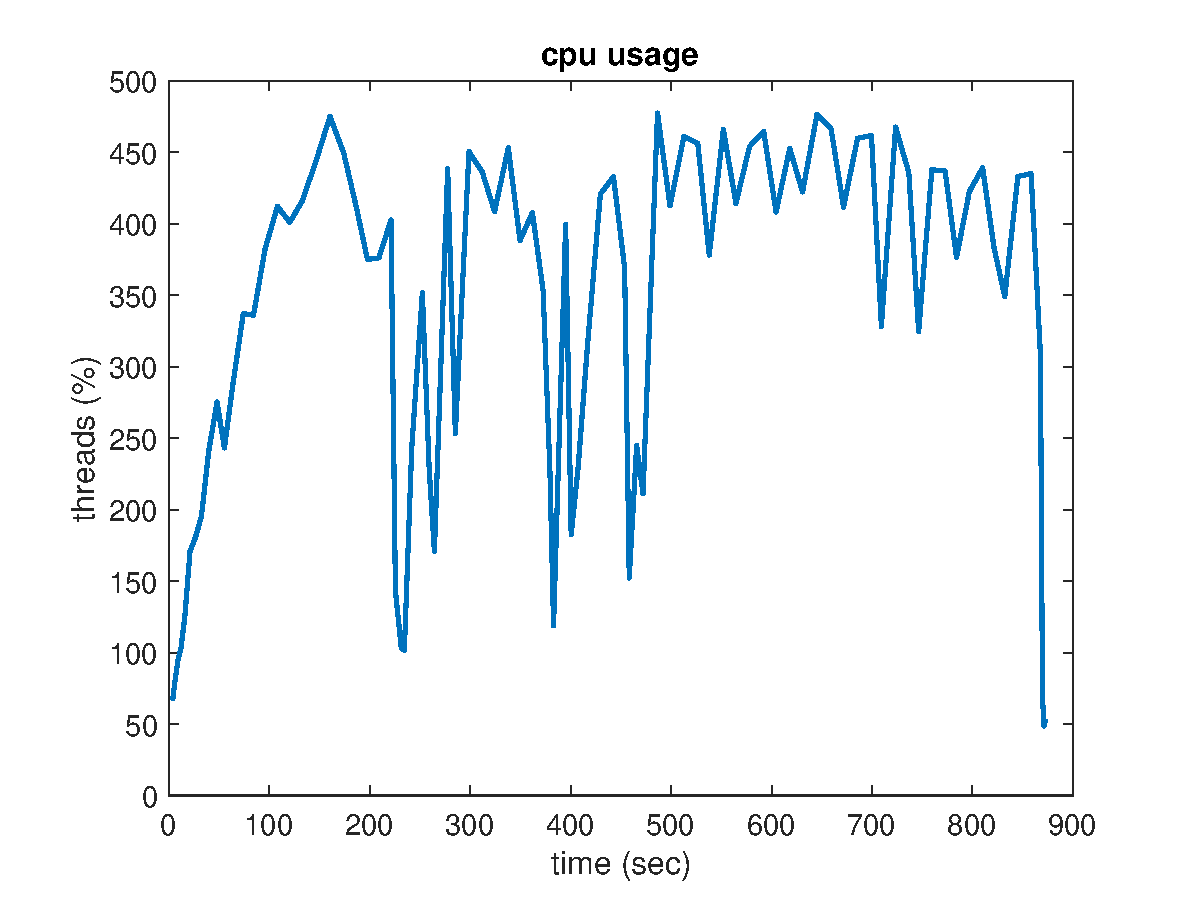
\includegraphics[width=0.9\textwidth]{fig/cartographer.eps}
  \end{center}
\end{frame}



\begin{frame}
  \frametitle{teb\_local\_planner usage (30Hz target frequency)}
  \begin{center}
    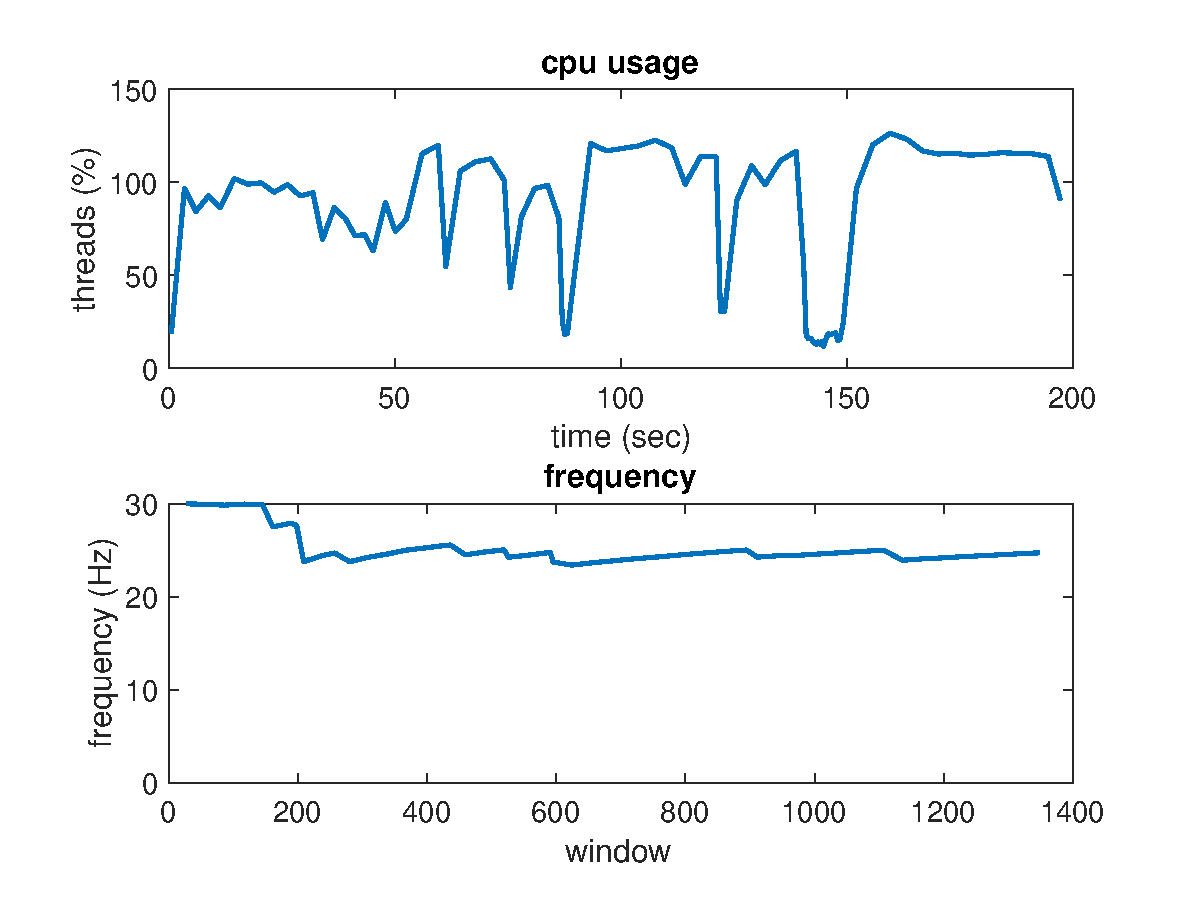
\includegraphics[width=0.9\textwidth]{fig/teb.eps}
  \end{center}
\end{frame}



\end{document}
